\begin{block}{4. System architecture}

  \begin{figure}
    \centering
    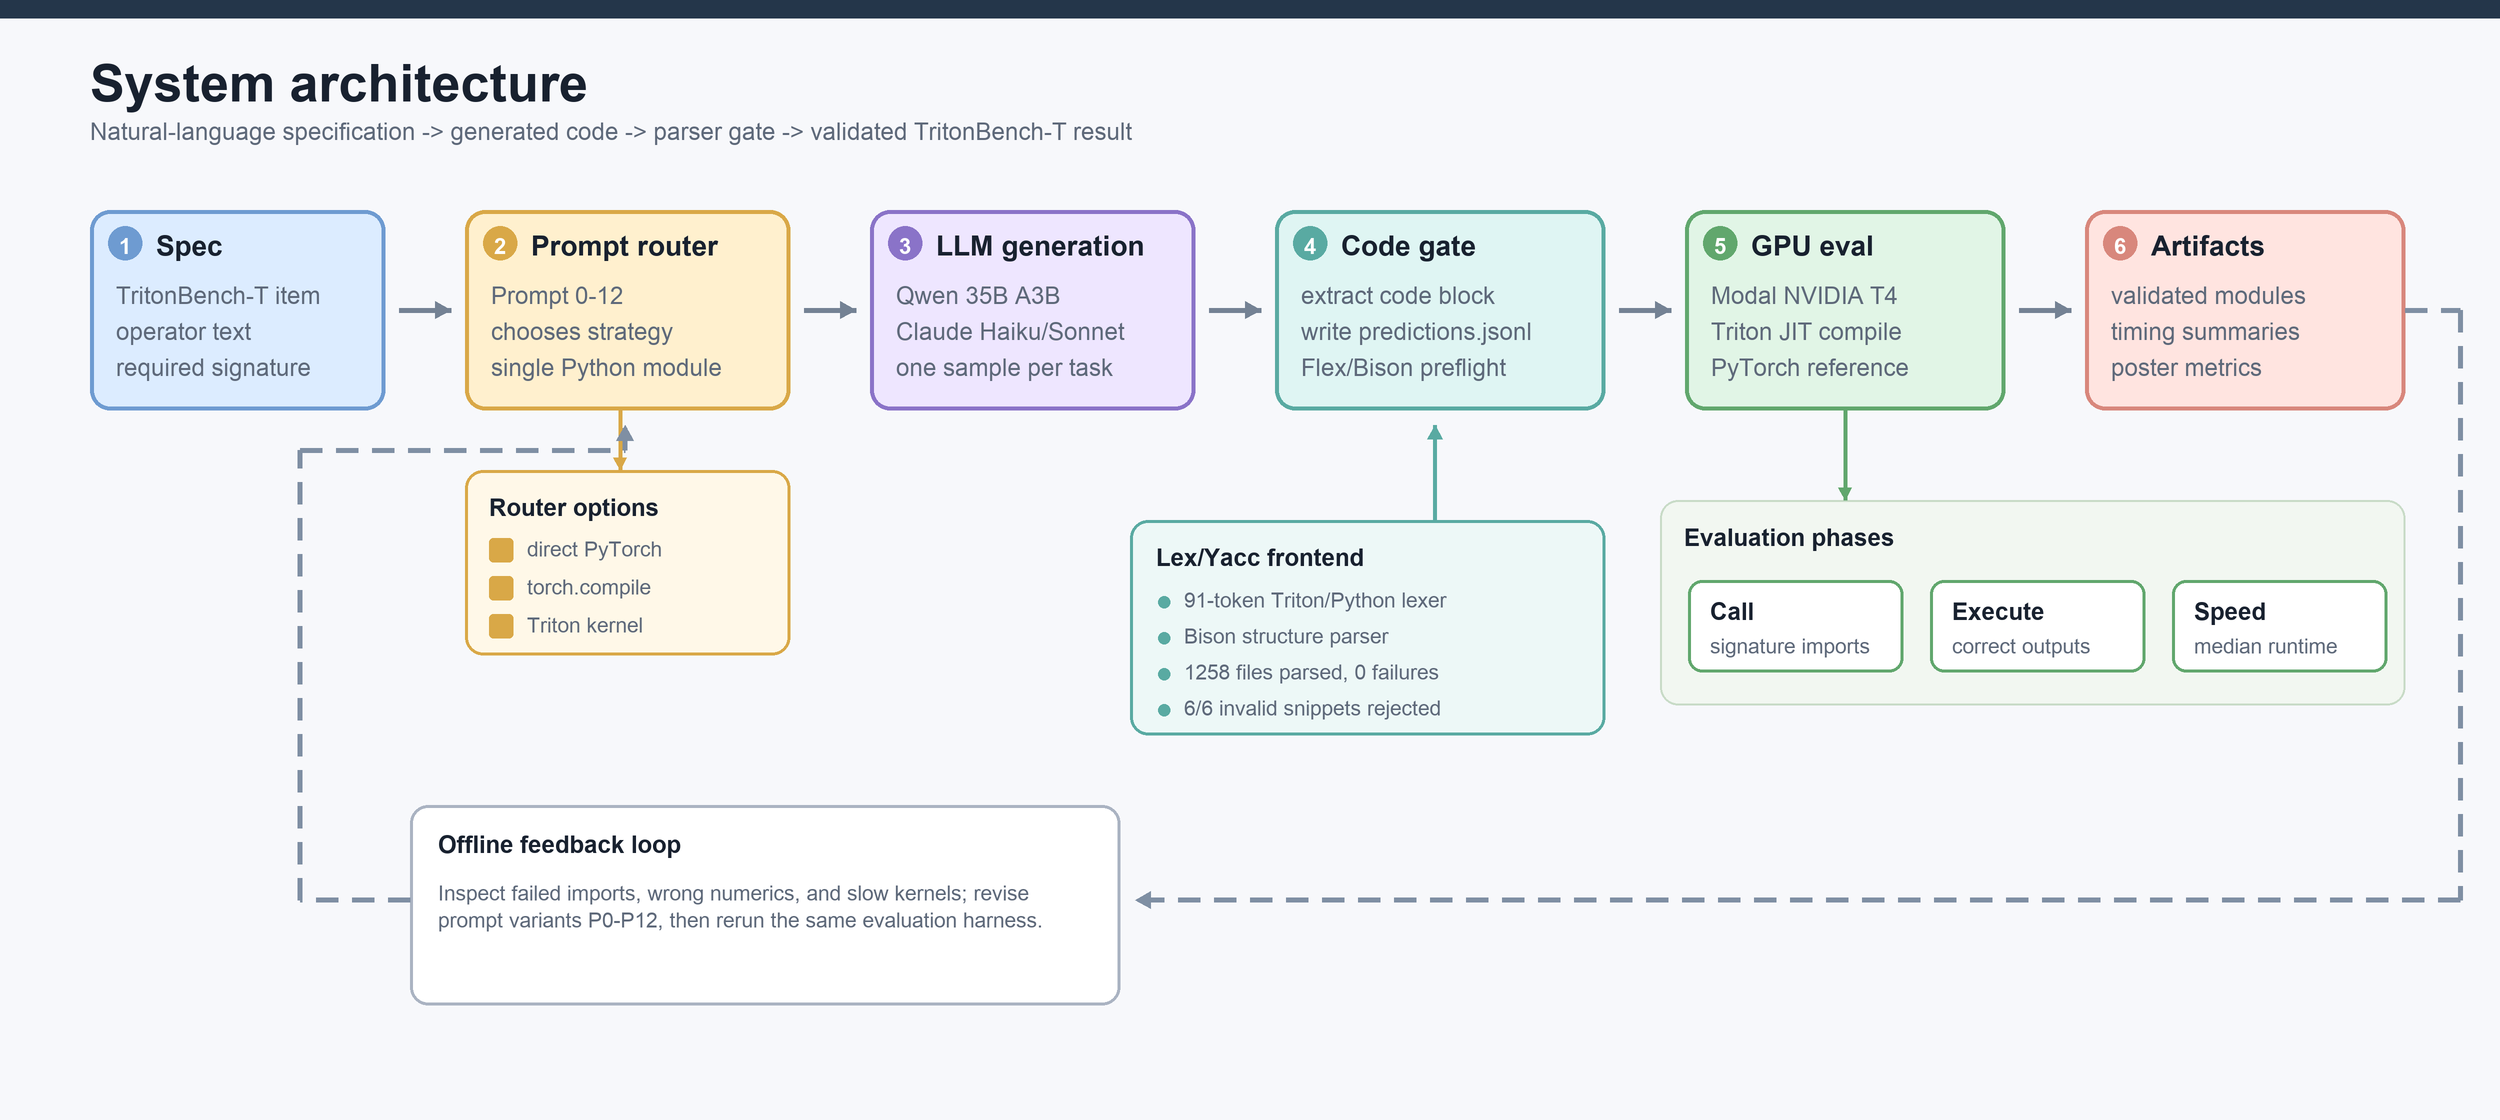
\includegraphics[width=0.97\textwidth]{figures/architecture.png}
    \caption{End-to-end pipeline from natural-language spec to validated TritonBench-T implementation.}
  \end{figure}

  Left to right, a TritonBench-T item provides the operator description and required wrapper signature. The prompt router builds a one-module request for Qwen or Claude and selects direct PyTorch, \texttt{torch.compile}, or Triton; the code extractor writes \texttt{predictions.jsonl} and the Lex/Yacc preflight rejects malformed Python/Triton before GPU evaluation. Modal then runs call, execution, and speed phases on an NVIDIA T4, archives surviving modules and metrics, and the failure summary feeds the next offline prompt revision.

\end{block}
